\section{Generalities}
\subsection{Power}
All primary displays use electrical power from the secondary AC bus.
The displays are turned on by the yellow top-left button on the TI
(\cockpitref{fig:front-panel}{item:TI}).
In addition, displays are turned on at takeoff when RPM exceeds 90\%.

The HUD requires 40 seconds of preheating after AC power is available, before turning on.

\section{Head Up Display (HUD)}
\subsection{Overview}
\begin{figure}[!ht]
  \centering
  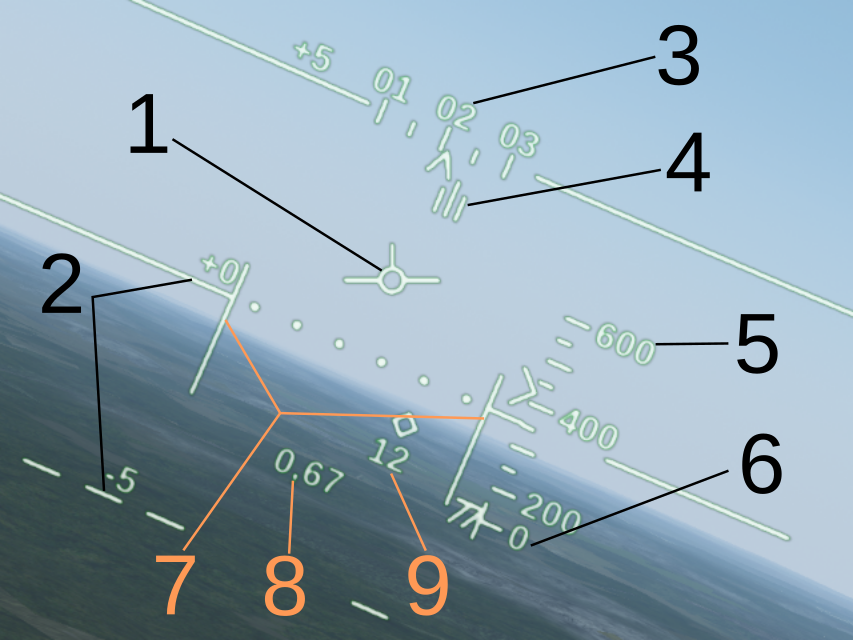
\includegraphics[width=0.7\textwidth]{images/displays/ja-hud-general.png}

  \begin{multicols}{2}
    \begin{enumerate}[nosep]
      \item \label{item:fpv} Flight path vector
      \item \label{item:horizon} Artificial horizon and pitch lines
      \item \label{item:heading} Heading scale
      \item \label{item:dest} Destination bearing
      \item \label{item:altitude} Altitude scale
      \item \label{item:rhm} Radar altimeter index and reference
      \item \label{item:altbars} Altitude bars
      \item \label{item:speed} Airspeed / Mach indicator
      \item \label{item:distance} Distance indicator
    \end{enumerate}
  \end{multicols}

  \caption{HUD overview}
  \label{fig:hud}
\end{figure}

\paragraph{Artificial Horizon (\cockpitref{fig:hud}{item:horizon})}
The artificial horizon and pitch scale provide an attitude reference.
The pitch scale consists of a line every 5 degrees.
Lines above the horizon are solid, lines below the horizon are dashed.
The artificial horizon itself is distinguished by six center dots.
Only the three pitch lines closest to the flight path vector are displayed.

\paragraph{Flight Path Vector (\cockpitref{fig:hud}{item:fpv})}
The FPV marker indicates the aircraft path direction relative to the ground.
Most of the HUD is centered around the FPV marker.

\paragraph{Heading Scale (\cockpitref{fig:hud}{item:heading})}
The heading scale is located above the FPV.
The fixed wedge index indicates aircraft track angle.
The second index consisting of 3 vertical lines
(\cockpitref{fig:hud}{item:dest}) indicates bearing to the next waypoint.

\paragraph{Altitude Scale (\cockpitref{fig:hud}{item:altitude})}
The altitude scale is located right of the FPV.
The fixed wedge index indicates aircraft altitude.
At low altitude the scale zooms in,
allowing to read the altitude more precisely for low level flight.

When the radar altimeter is active and in range,
the altitude 0 mark is displayed just below the altitude scale
(\cockpitref{fig:hud}{item:rhm}).
The radar altitude index, consisting of two wedges, can be read against this mark.
This can be used to set the altimeter QFE in flight.

\paragraph{Altitude Bars (\cockpitref{fig:hud}{item:altbars})}
The two altitude bars indicate the reference altitude
(also called commanded altitude) relative to the current altitude.

The top of the altitude bars represents commanded altitude,
while the artificial horizon represents current altitude.
If the top of the bars is on the horizon, the aircraft is at the commanded altitude.
If the top of the bars is above (resp.\ below) the horizon,
the aircraft is below (resp.\ above) the commanded altitude.

When the FPV is within 1\textdegree{} of the horizon,
the altitude scale index is fixed on the horizon.
Under these conditions, the top of the altitude bars
can be read on the altitude scale to obtain the commanded altitude.

Altitude bars are only displayed below 1000m.
When autopilot altitude hold is active, boxes are displayed together with
(below 1000m) or instead of (above 1000m) the altitude bars.

\subparagraph{Reference Altitude}
\label{sec:ref-alt}
The reference altitude displayed by the altitude bars is set as follows.
\begin{itemize}[noitemsep]
  \item During takeoff, the altitude bars are fixed over the horizon.
    After leaving takeoff mode, reference altitude is set to 500m.
  \item During flight, the reference button (keybinding \keys{\shift+R})
    sets the reference altitude to the current altitude.
  \item If autopilot altitude hold mode is active,
    the reference altitude is the autopilot altitude.
  \item When entering landing mode, reference altitude is set to 500m.
    It can still be modified with the reference button or by engaging autopilot altitude hold.
\end{itemize}

\paragraph{Airspeed / Mach Indicator (\cockpitref{fig:hud}{item:speed})}
Digital airspeed is displayed below the FPV,
with a minimum of 75km/h and a precision of 5km/h
(40kts and 1kts respectively in imperial units mode).
Above M 0.5, airspeed is replaced by a Mach indicator.

\paragraph{Distance Indicator (\cockpitref{fig:hud}{item:distance})}
Displays digital distance to the next waypoint.

\paragraph{Radar Altitude}
When radar altitude is less than 100m, it is displayed digitally
in the lower left part of the HUD, with the format e.g.\ `R 45'.
It is hidden for 30s after exiting takeoff mode, and in landing mode.

\paragraph{Ground Collision Warning}
Ground collision warning is displayed on the HUD as
a flashing arrow over the FPV, pointing in the pull-up direction.

\paragraph{Text Indications}
To the lower left of the FPV, plain text indications
can be shown in the following priority order:
\begin{enumerate}
  \item Altimeter setting warning `QFE' (flashing).
    At takeoff, indicates that the altimeter is incorrectly set.
    In flight, indicates that the altimeter should be switched to/from STD mode
    (assumes transition altitude 1500m).
  \item In landing mode, `TILS' indication when receiving ILS signal.
    (flashing if glideslope is not available or not in range).
  \item Selected weapon type (at the earliest 30s after leaving takeoff mode).
\end{enumerate}


\subsection{Takeoff Mode}
\begin{figure}[!ht]
  \centering
  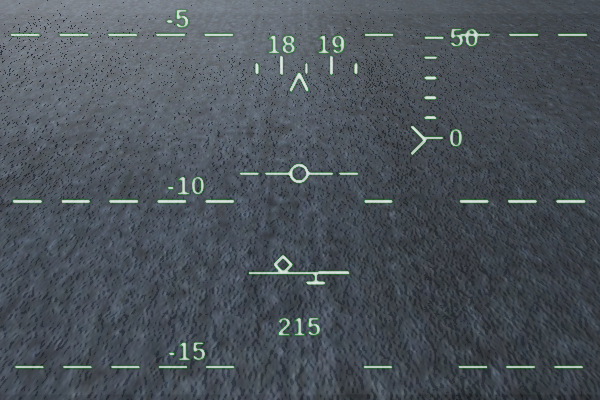
\includegraphics[width=0.5\textwidth]{images/displays/ja-hud-takeoff.png}
  \caption{HUD during takeoff}
  \label{fig:hud-takeoff}
\end{figure}

Takeoff mode is enabled when the nose gear is compressed.

During takeoff, the FPV is fixed vertically 10\textdegree{}
below the aircraft forward axis, and its symbol changes.
Horizontally, the FPV functions as in navigation mode,
and will e.g.\ move due to sidewind after rotation.

The distance line is displayed below the FPV, and represents airspeed.
The diamond upper index indicates aircraft speed,
and the inverted-T bottom marker indicates recommended rotation speed.
When the rotation angle reaches 5\textdegree{}, the distance line is hidden.

Takeoff mode stops once the airspeed exceeds M 0.35,
when the climb angle is at least 3\textdegree{},
or at landing gear retraction.

\subsection{Landing Mode}
\begin{figure}[!ht]
  \centering
  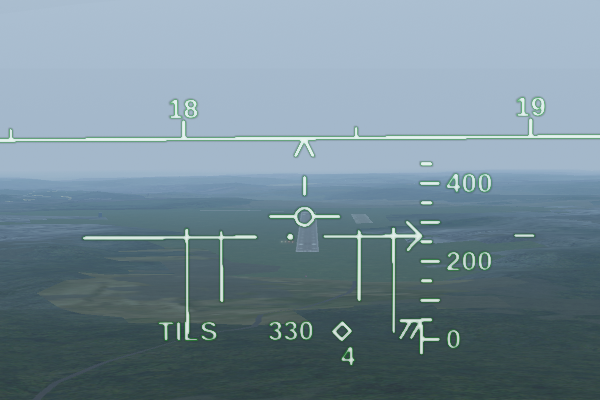
\includegraphics[width=0.5\textwidth]{images/displays/ja-hud-landing.png}
  \caption{HUD during final}
  \label{fig:hud-landing}
\end{figure}

In landing mode, the HUD changes when starting the final.
The -5\textdegree{} pitch line is removed,
and a glideslope line is added 2.86\textdegree{} below the horizon
(corresponding to a slope of 5\%).
Altitude scale, digital airspeed, and distance indicator are positioned around the glideslope line.
Heading scale is positioned over the horizon, and changes to a 1:1 scale.
Altitude bars are hidden.

If the climb or dive angle exceeds $\pm 7.5\degree$,
the default presentation of the pitch scale, digital airspeed, and distance indicator is restored,
while the heading and altitude scales are hidden.

\paragraph{Speed / AoA Indicator}
In landing mode, the vertical fin (`tail') of the flight path vector symbol
moves vertically to indicate deviation from the target speed or angle of attack.

The speed is correct when the bottom of the tail is on the FPV circle
(default position in navigation mode).
If the tail is higher than the circle, the aircraft speed is too high.
If the tail is lower (inside the circle), the aircraft speed is too low.

While the landing gear is up, the target speed is 550km/h.
Once the landing gear is down and locked, the target angle of attack is
computed based on aircraft weight, with a maximum of 12\textdegree{}
(15.5\textdegree{} if the button \cockpitref{fig:front-panel}{item:autothrottle-lights} is pressed and lit).

When the landing gear is down, the fin will blink if the angle of attack is critically high.

\paragraph{ILS Guidance}
If ILS guidance is used, the reference point on the glideslope line
indicates the heading to follow to align with the localizer.
Four vertical bars on the glideslope line indicate ILS glideslope deviation:
if the top of the bars is above, resp.\ below the glideslope line,
the aircraft is below, resp.\ above the ILS glideslope.

If ILS is not used (optical landing mode),
the reference point is aligned with the FPV, and the vertical bars are hidden.

\paragraph{Touchdown}
Below 35m, the HUD switches to optical landing display (ILS indications disappear).
Below 15m radar altitude, the HUD switches to flare mode.
The glideslope line moves up to indicate the descent angle
which gives a vertical speed of 2.8m/s, the maximum for touchdown.
If radar altitude is unavailable, transition to flare mode occurs at 35m.

Once the nose gear is compressed, the HUD switches to takeoff mode.

\subsection{Tactical Information}
Some tactical information is displayed on the HUD when a weapon is selected,
when a radar contact is tracked, and while in aiming mode.
%See \cref{chap:weapons} for details.
